\documentclass[12pt]{article}
\usepackage[utf8]{inputenc}

\usepackage{amsfonts}
\usepackage{amsmath}
\usepackage{amssymb}
\PassOptionsToPackage{hyphens}{url}
\usepackage{hyperref}
\usepackage{wasysym}
\usepackage{graphicx}
\usepackage{multicol}
\usepackage[title]{appendix}

\usepackage{geometry}
\geometry{a4paper,scale=0.8}

\usepackage{pdfrender,xcolor}
\pdfrender{StrokeColor=black,TextRenderingMode=2,LineWidth=0.2pt}

\usepackage{import}

\begin{document}

% Titlepage
\begin{titlepage}

\begin{center}
    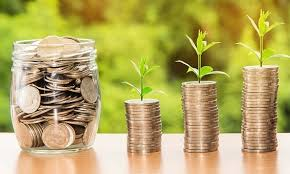
\includegraphics[width=15cm]{./titlepage.jpeg}
    
    \vspace*{1cm}

    \textbf{\Huge \bfseries Business Report}
            
    \vspace{1.5cm}

    \textbf{\large Jue Gong, Xinyi Qian}

    \vfill
    
    \textbf{February 2022\\
    Hymans Robertson LLP}
\end{center}

\end{titlepage}

%\maketitle

\newpage

\tableofcontents
\newpage

\import{./}{section1.tex}

\import{./}{section2.tex}

\import{./}{section3.tex}

\import{./}{section4.tex}

\import{./}{section5.tex}

\import{./}{section6.tex}

\begin{appendices}
\section{Related Links}
Since our datasets regarding stock returns and covariance are too large which are not suitable to display in our document, we create a GitHub repository to store them. Also we have uploaded our model for this competition, called Folio.dat and Folio.mos compiled by Xpress. More details see link: \url{https://github.com/Candlelight-Edin/Undergraduate-Operational-Research-Challenge}.
\end{appendices}

\end{document}